\documentclass[aspectratio=169,11pt]{beamer}

\definecolor{customblue}{rgb}{0.13,0.28,0.59}
\definecolor{accentorange}{rgb}{0.88,0.32,0.12}
\definecolor{mutedgreen}{rgb}{0.10,0.55,0.35}
\setbeamercolor{block title}{bg=customblue,fg=white}
\setbeamercolor{block body}{bg=customblue!8}
\setbeamercolor{alerted text}{fg=accentorange}
\setbeamertemplate{blocks}[rounded]
\usepackage{amsmath,booktabs,graphicx,tikz}
\usetikzlibrary{arrows.meta,positioning}
% Traditional presentation definitions shared with the update-slide template.
\newcommand{\BEAS}{\begin{eqnarray*}}
\newcommand{\EEAS}{\end{eqnarray*}}
\newcommand{\BEA}{\begin{eqnarray}}
\newcommand{\EEA}{\end{eqnarray}}
\newcommand{\BEQ}{\begin{equation}}
\newcommand{\EEQ}{\end{equation}}
\newcommand{\BIT}{\begin{itemize}}
\newcommand{\EIT}{\end{itemize}}
\newcommand{\BNUM}{\begin{enumerate}}
\newcommand{\ENUM}{\end{enumerate}}
\newcommand{\BF}{\begin{frame}}
\newcommand{\EF}{\end{frame}}

\newcommand{\argmin}{\mathop{\rm argmin}}
\newcommand{\sign}{\mathop{\rm sign}}

\newcommand{\cf}{{\it cf.}}
\newcommand{\eg}{{\it e.g.}}
\newcommand{\ie}{{\it i.e.}}
\newcommand{\etc}{{\it etc.}}

\newcommand{\ones}{\mathbf 1}

\newcommand{\reals}{{\mbox{\bf R}}}
\newcommand{\integers}{{\mbox{\bf Z}}}
\newcommand{\complex}{{\mbox{\bf C}}}
\newcommand{\symm}{{\mbox{\bf S}}}

\newcommand{\Span}{\mbox{\textrm{span}}}
\newcommand{\Range}{\mbox{\textrm{range}}}
\newcommand{\nullspace}{{\mathcal N}}
\newcommand{\range}{{\mathcal R}}
\newcommand{\Nullspace}{\mbox{\textrm{nullspace}}}
\newcommand{\Rank}{\mathop{\bf Rank}}
\newcommand{\Card}{\mathop{\bf Card}}
\newcommand{\Tr}{\mathop{\bf Tr}}
\newcommand{\diag}{\mathop{\bf diag}}
\newcommand{\lambdamax}{{\lambda_{\rm max}}}
\newcommand{\lambdamin}{\lambda_{\rm min}}

\newcommand{\Expect}{\mathop{\bf E{}}}
\newcommand{\Prob}{\mathop{\bf Prob}}
\newcommand{\erf}{\mathop{\bf erf}}


\mode<presentation>{\usetheme{default}}
\usecolortheme[rgb={0.13,0.28,0.59}]{structure}
\setbeamertemplate{navigation symbols}{}
\setbeamertemplate{itemize subitem}{--}
\setbeamertemplate{footline}{%
  \begin{beamercolorbox}[ht=2.5ex,dp=1.125ex,leftskip=.8cm,rightskip=.6cm]{structure}
    \hfill\insertframenumber
  \end{beamercolorbox}\vskip0.25cm
}

\graphicspath{{../../experiments/}}
\newcommand{\tightitems}{\setlength{\itemsep}{0.42em}}
\newcommand{\done}{\textcolor{mutedgreen}{\textbf{Complete}}}
\newcommand{\open}{\textcolor{accentorange}{\textbf{Open}}}

\title{CVXOPF: multiscale optimization for battery resilience}
\subtitle{From nonlinear power flow to month-scale hierarchical control}
\author{Bennet Meyers}
\date{August 26, 2026}

\begin{document}

\begin{frame}
  \titlepage
\end{frame}

\begin{frame}{The research goal}
  \textbf{How can we plan battery energy over long horizons while respecting
  the nonlinear AC network physics that determine whether each action is realizable?}
  \vspace{0.7em}
  \begin{columns}[T,onlytextwidth]
    \column{0.48\textwidth}
    \textbf{Long-horizon decisions}
      \begin{itemize}\tightitems
        \item energy adequacy and terminal reserves
        \item renewable curtailment and load service
        \item storage cycling across days to seasons
      \end{itemize}
    \column{0.48\textwidth}
    \textbf{Short-horizon physics}
      \begin{itemize}\tightitems
        \item voltage and reactive-power feasibility
        \item two-terminal branch ratings and losses
        \item nonconvex AC solver behavior
      \end{itemize}
  \end{columns}
  \vspace{0.4em}
  \centering\large The project thesis: \textbf{plan energy globally; realize power flow locally.}
\end{frame}

\begin{frame}{Why intertemporal optimization matters}
  \begin{columns}[c,onlytextwidth]
    \column{0.57\textwidth}
    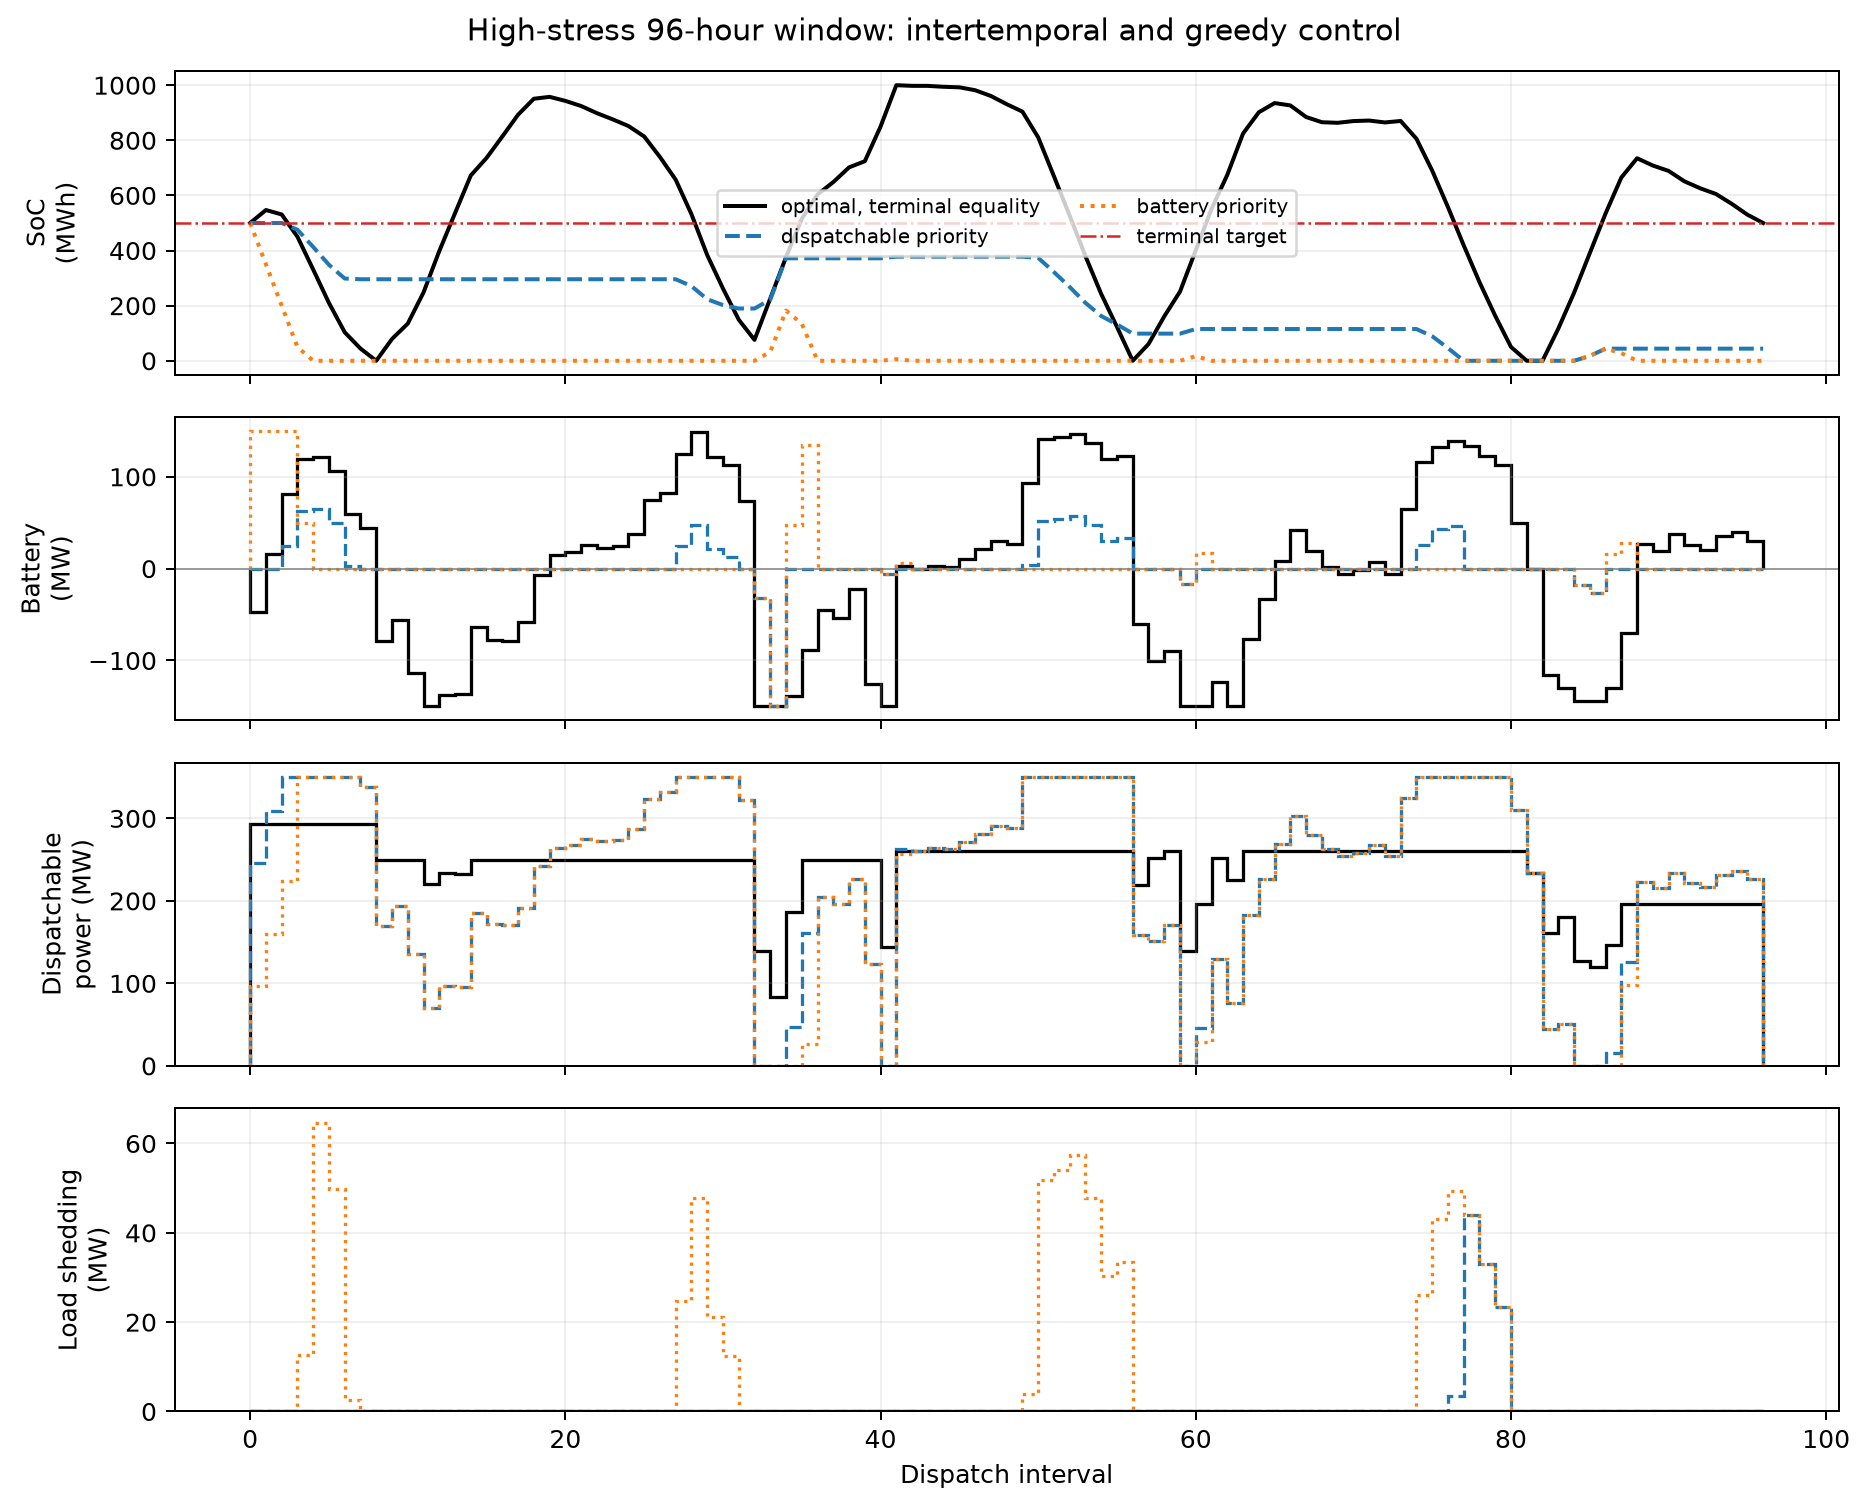
\includegraphics[width=\textwidth,height=0.69\textheight,keepaspectratio]{../../experiments/battery_terminal/readme_intertemporal_storage.png}
    \column{0.40\textwidth}
    \begin{itemize}\tightitems
      \item High-stress 96-hour case9: optimal control versus two terminal-blind greedy policies.
      \item The optimizer coordinates renewables, dispatch, and stored energy across four days.
      \item A hard terminal policy returns the battery to 500 MWh.
      \item Greedy policies exhaust or strand energy—and shed load.
    \end{itemize}
  \end{columns}
\end{frame}

\begin{frame}{A common modeling system now spans the research questions}
  \small
  \begin{center}
  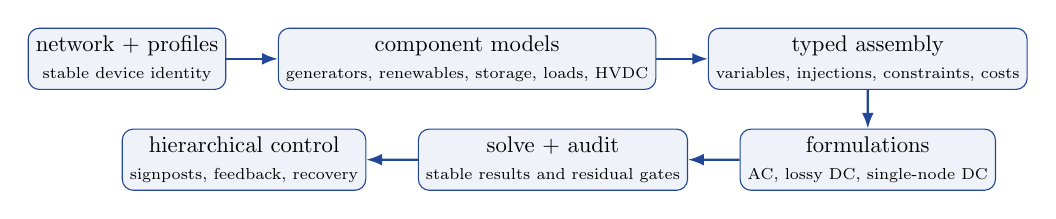
\begin{tikzpicture}[scale=0.82,transform shape,node distance=6mm and 8mm,
    box/.style={draw=customblue,rounded corners,fill=customblue!7,minimum height=9mm,align=center},
    arr/.style={-{Latex[length=2mm]},thick,customblue}]
    \node[box] (data) {network + profiles\\\scriptsize stable device identity};
    \node[box,right=of data] (components) {component models\\\scriptsize generators, renewables, storage, loads, HVDC};
    \node[box,right=of components] (assembly) {typed assembly\\\scriptsize variables, injections, constraints, costs};
    \node[box,below=of assembly] (forms) {formulations\\\scriptsize AC, lossy DC, single-node DC};
    \node[box,left=of forms] (solve) {solve + audit\\\scriptsize stable results and residual gates};
    \node[box,left=of solve] (hier) {hierarchical control\\\scriptsize signposts, feedback, recovery};
    \draw[arr] (data)--(components); \draw[arr] (components)--(assembly);
    \draw[arr] (assembly)--(forms); \draw[arr] (forms)--(solve); \draw[arr] (solve)--(hier);
  \end{tikzpicture}
  \end{center}
  \begin{itemize}
    \item Components contribute their own mathematics through a typed contract.
    \item Formulation builders aggregate those contributions generically, so storage, load, and network semantics survive across layers.
  \end{itemize}
\end{frame}

\begin{frame}[shrink=5]{What the software can model today}
  \small
  \begin{columns}[T,onlytextwidth]
    \column{0.48\textwidth}
    \begin{block}{Network and formulations}
      \begin{itemize}\tightitems
        \item nonlinear AC OPF through CVXPY DNLP/IPOPT
        \item convex lossy-DC and single-node formulations
        \item active branch status and two-terminal AC thermal limits
        \item sparse and dense network representations
      \end{itemize}
    \end{block}
    \begin{block}{Intertemporal control}
      \begin{itemize}\tightitems
        \item single- and multistep problems
        \item hard, shortfall, and soft terminal policies
        \item public hierarchical DC--AC orchestration
      \end{itemize}
    \end{block}
    \column{0.48\textwidth}
    \begin{block}{First-class components}
      \begin{itemize}\tightitems
        \item dispatchable and nondispatchable generation
        \item batteries with real/reactive capability and cycling cost
        \item fixed and economically sheddable loads
        \item lossy controllable HVDC links
      \end{itemize}
    \end{block}
    \begin{block}{Research discipline}
      \begin{itemize}\tightitems
        \item typed identities and stable failure schemas
        \item explicit objective time units
        \item retained audit residuals and reproducible experiments
      \end{itemize}
    \end{block}
  \end{columns}
\end{frame}

\begin{frame}[shrink=3]{Equivalent mathematics can have radically different numerical behavior}
  \centering
  \includegraphics[width=0.98\textwidth,height=0.68\textheight,keepaspectratio]{formulation_results.pdf}
  \begin{itemize}\small\tightitems
    \item Direct and lifted branch-terminal equations agree below $4.5\times10^{-14}$ p.u.; paired objectives agree to solver precision.
    \item Lifting adds variables and equalities but separates nonlinear voltage expressions from quadratic thermal inequalities.
    \item On case57, the lifted structure was 27$\times$ faster in sparse form and 110$\times$ faster in dense form.
  \end{itemize}
\end{frame}

\begin{frame}{Terminal energy is an economic decision, not a boundary detail}
  \centering
  \includegraphics[width=0.98\textwidth,height=0.68\textheight,keepaspectratio]{terminal_policy_results.pdf}
  \begin{itemize}\small\tightitems
    \item The sampled fixed-terminal value is empirically convex and piecewise smooth.
    \item Linear penalties recover a hard target beyond a marginal-value threshold; quadratic penalties create a smooth tradeoff.
    \item Terminal policy therefore encodes the value or obligation attached to energy beyond the modeled horizon.
  \end{itemize}
\end{frame}

\begin{frame}{Long-horizon energy states can coordinate short-horizon AC solves}
  \centering
  \includegraphics[width=0.98\textwidth,height=0.68\textheight,keepaspectratio]{locality_and_handoff.pdf}
  \begin{itemize}\small\tightitems
    \item Terminal influence remains concentrated in a final coupled excursion as the planning horizon grows.
    \item Endpoint-fixed AC subsections reach energy boundaries inherited from the long DC solution while choosing their own network-feasible trajectories.
  \end{itemize}
\end{frame}

\begin{frame}{The hierarchical controller closes the loop}
  \centering
  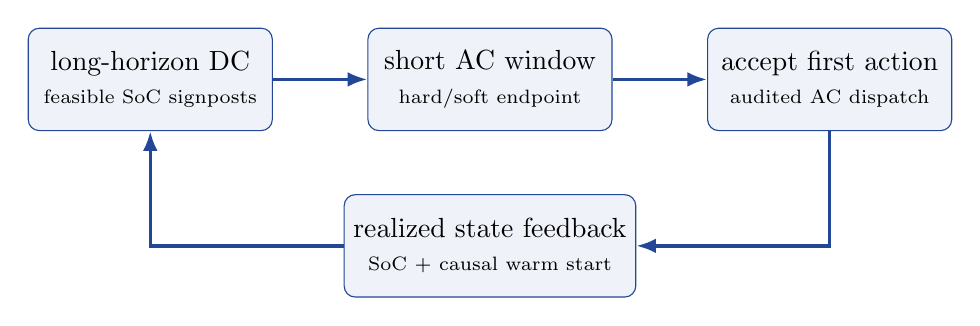
\begin{tikzpicture}[node distance=8mm and 12mm,
    box/.style={draw=customblue,rounded corners,fill=customblue!7,minimum width=31mm,minimum height=13mm,align=center},
    arr/.style={-{Latex[length=2.5mm]},very thick,customblue}]
    \node[box] (outer) {long-horizon DC\\\scriptsize feasible SoC signposts};
    \node[box,right=of outer] (window) {short AC window\\\scriptsize hard/soft endpoint};
    \node[box,right=of window] (action) {accept first action\\\scriptsize audited AC dispatch};
    \node[box,below=of window] (state) {realized state feedback\\\scriptsize SoC + causal warm start};
    \draw[arr] (outer)--(window); \draw[arr] (window)--(action);
    \draw[arr] (action)|-(state); \draw[arr] (state)-|(outer);
  \end{tikzpicture}
  \vspace{1em}
  \begin{itemize}\tightitems
    \item The outer model maintains the energy plan; the inner model realizes the next action with AC voltage, reactive-power, loss, and thermal physics.
    \item Realized state—not an imagined DC action—feeds the next decision.
  \end{itemize}
\end{frame}

\begin{frame}{The first 96-hour study exposed two different failure mechanisms}
  \centering
  \includegraphics[width=0.92\textwidth,height=0.55\textheight,keepaspectratio]{m17_policy_outcomes.pdf}
  \begin{itemize}\tightitems
    \item \textbf{Numerical/local-solver sensitivity:} flat-start IPOPT reported infeasible at one hard-target window; six alternate starts solved the identical problem.
    \item \textbf{Genuine loss of terminal viability:} soft deviations left 128.1 MW required charging in the last hour, but only 123.6 MW aggregate headroom.
  \end{itemize}
\end{frame}

\begin{frame}{Causal initialization recovery works in the reference scenario}
  \begin{columns}[T,onlytextwidth]
    \column{0.58\textwidth}
    \textbf{Frozen 96-hour recovery experiment}
      \begin{itemize}\tightitems
        \item 96/96 intervals completed with hard AC endpoints.
        \item Shifted preceding AC solution succeeded on 94/95 later windows (98.9\%).
        \item The one failed audit recovered through a target-free solve followed by a copied hard-target solve.
        \item 98 AC solves total; no perturbation attempts needed.
      \end{itemize}
    \column{0.38\textwidth}
    \textbf{Interpretation}
    \begin{itemize}\tightitems
      \item Warm starts are part of the operational method, not merely a speed hint.
      \item A local solver status is not a physical infeasibility certificate.
      \item M17 subsequently matched the frozen manual reference across all four policy cases with zero failed comparisons.
    \end{itemize}
  \end{columns}
\end{frame}

\begin{frame}{Case118 makes the computational boundary visible}
  \begin{columns}[T,onlytextwidth]
    \column{0.54\textwidth}
    \textbf{Six-hour rated AC pilot}
      \begin{itemize}\tightitems
        \item 205.9 MW maximum storage movement
        \item 465.8 MWh battery throughput
        \item thermally binding accepted solution
        \item 34.5 minute solve
        \item 14.66 GiB peak process RSS
      \end{itemize}
    \column{0.42\textwidth}
    \begin{itemize}\tightitems
      \item \textbf{Scientifically,} the battery is active and network-constrained—not an inert device in a large network.
      \item \textbf{Computationally,} direct 24-hour or annual AC optimization is not a responsible baseline on this stack.
    \end{itemize}
  \end{columns}
\end{frame}

\begin{frame}{The hierarchy has progressed from hours to a month}
  \small
  \begin{center}
  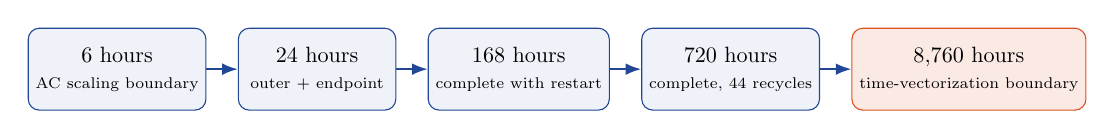
\begin{tikzpicture}[scale=0.80,transform shape,node distance=5mm,
    stage/.style={draw=customblue,rounded corners,minimum width=25mm,minimum height=13mm,align=center,fill=customblue!7},
    arr/.style={-{Latex[length=2mm]},thick,customblue}]
    \node[stage] (pilot) {6 hours\\\scriptsize AC scaling boundary};
    \node[stage,right=of pilot] (day) {24 hours\\\scriptsize outer + endpoint};
    \node[stage,right=of day] (week) {168 hours\\\scriptsize complete with restart};
    \node[stage,right=of week] (month) {720 hours\\\scriptsize complete, 44 recycles};
    \node[stage,right=of month,fill=accentorange!12,draw=accentorange] (year) {8,760 hours\\\scriptsize time-vectorization boundary};
    \draw[arr] (pilot)--(day); \draw[arr] (day)--(week); \draw[arr] (week)--(month); \draw[arr] (month)--(year);
  \end{tikzpicture}
  \end{center}
  \vspace{0.8em}
  \begin{itemize}\tightitems
    \item Week: 168/168 accepted intervals; the 16 GiB supervisor stopped safely at 128 and a fresh continuation completed the trajectory.
    \item Month: 720/720 accepted intervals; three copied-target-free recoveries; maximum external RSS 15.99 GiB.
    \item Tail latency: a predeclared 300-second primary budget plus causal recovery reduced latency on all three observed slow-success windows.
  \end{itemize}
\end{frame}

\begin{frame}{Process recycling controls memory without changing the science}
  \centering
  \includegraphics[width=0.98\textwidth,height=0.69\textheight,keepaspectratio]{recycling_memory.pdf}
  \begin{itemize}\small\tightitems
    \item All three 64-interval arms completed with identical causal trajectories.
    \item Peak external RSS fell from 20.03 GiB (never) to 17.93 GiB (recycle every 16).
    \item Fresh-process execution is now an explicit part of the scalable experimental method.
  \end{itemize}
\end{frame}

\begin{frame}{The annual study separates planning, partitioning, and execution}
  \centering
  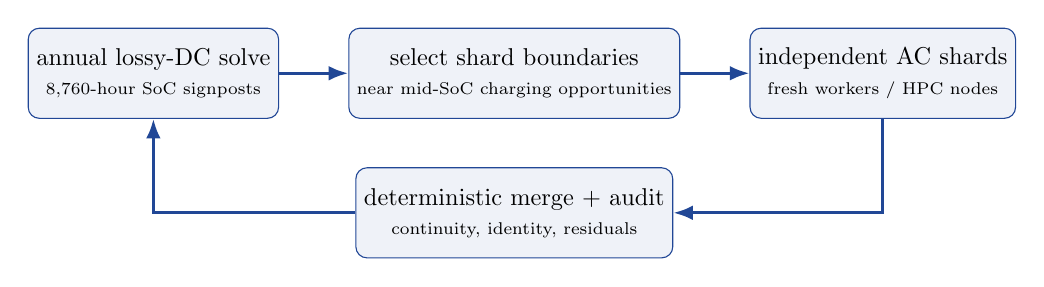
\begin{tikzpicture}[scale=0.88,transform shape,node distance=7mm and 10mm,
    box/.style={draw=customblue,rounded corners,fill=customblue!7,minimum width=30mm,minimum height=13mm,align=center},
    arr/.style={-{Latex[length=2.5mm]},very thick,customblue}]
    \node[box] (dc) {annual lossy-DC solve\\\scriptsize 8,760-hour SoC signposts};
    \node[box,right=of dc] (cut) {select shard boundaries\\\scriptsize near mid-SoC charging opportunities};
    \node[box,right=of cut] (ac) {independent AC shards\\\scriptsize fresh workers / HPC nodes};
    \node[box,below=of cut] (merge) {deterministic merge + audit\\\scriptsize continuity, identity, residuals};
    \draw[arr] (dc)--(cut); \draw[arr] (cut)--(ac); \draw[arr] (ac)|-(merge); \draw[arr] (merge)-|(dc);
  \end{tikzpicture}
  \vspace{1em}
  \begin{itemize}\tightitems
    \item The supervised annual outer-only S4 gate is implemented, reviewed, and committed—but the existing per-step CVXPY graph did not fit the machine.
    \item macOS killed the detached worker at the same late construction/canonicalization phase: sampled RSS was 11.69 GiB, while the kernel reported 198,602 MB for the largest compressed process.
    \item The experiment is paused for M14 time vectorization; an accepted outer trajectory will still determine—not be tuned by—the later sharding qualification.
  \end{itemize}
\end{frame}

\begin{frame}{Annual failure identifies the next milestone}
  \begin{columns}[T,onlytextwidth]
    \column{0.50\textwidth}
    \textbf{What the failed workers established}
      \begin{itemize}\tightitems
        \item No outer primal or annual signpost artifact was produced.
        \item The experiment supervisor triggered neither its 16 GiB RSS limit nor its wall-time limits.
        \item A launchd-owned retry ruled out the Codex command resource group and presentation edits.
        \item The event is a construction/canonicalization resource boundary—not infeasibility.
      \end{itemize}
    \column{0.46\textwidth}
    \textbf{M14: vectorize time}
      \begin{itemize}\tightitems
        \item time-indexed matrix variables
        \item batched network/component constraints
        \item sparse storage-difference operators
        \item vectorized costs and reporting
        \item short-horizon equivalence before annual rerun
      \end{itemize}
  \end{columns}
\end{frame}

\begin{frame}{What we have learned}
  \begin{enumerate}\tightitems
    \item \textbf{Model structure matters computationally.} Equivalent nonlinear formulations can differ by orders of magnitude in tractability.
    \item \textbf{Terminal energy is part of the scientific model.} Hard obligations, reserve floors, and soft value functions answer different questions.
    \item \textbf{DC signposts can coordinate AC realizations.} The layers need shared state, not identical trajectories.
    \item \textbf{Feedback is not recursive feasibility.} Soft deviations can consume the remaining ability to satisfy a terminal obligation.
    \item \textbf{Solver recovery is operationally relevant.} Causal warm starts distinguish numerical failure from demonstrated physical infeasibility.
    \item \textbf{Scaling requires both algebra and systems engineering.} Time-vectorized graphs, supervision, immutable artifacts, recycling, and sharding are part of doing the science correctly.
  \end{enumerate}
\end{frame}

\begin{frame}{Next steps}
  \begin{columns}[T,onlytextwidth]
    \column{0.48\textwidth}
    \textbf{Immediate Case118 path}
      \begin{enumerate}\tightitems
        \item complete M14 lossy-DC time vectorization
        \item rerun and analyze annual outer S4
        \item freeze and qualify shard boundaries
        \item run and merge the annual AC hierarchy
      \end{enumerate}
    \column{0.48\textwidth}
    \textbf{Research extensions}
      \begin{itemize}\tightitems
        \item recursive-feasibility protection with load shedding
        \item configurable multi-layer hierarchies
        \item SOCP as a possible middle layer
        \item uncertainty, contingencies, and storage siting/sizing
        \item reactive-support selection and pricing questions
      \end{itemize}
  \end{columns}
\end{frame}

\appendix

\begin{frame}{Appendix: load shedding is now a first-class reliability decision}
  \begin{itemize}\tightitems
    \item Loads have stable identities, fixed active/reactive demand, optional shedding eligibility, fractional caps, and VOLL-like costs.
    \item The model reports served load, shed load, fraction shed, energy not served, and integrated shedding cost.
    \item In the controlled single-node case, shedding below the relevant generator marginal cost and full service above it produce the expected economic phase transition.
    \item Explicit time-varying inequalities and leaf-bound representations agreed to solver precision; explicit inequalities were retained for clarity and uniformity.
  \end{itemize}
\end{frame}

\begin{frame}{Appendix: scientific boundaries}
  \small
  \begin{itemize}\tightitems
    \item AC results are accepted local solutions from CVXPY DNLP/IPOPT, not global-optimality certificates.
    \item Results establish behavior for the frozen case9/Tracy and synthetic Case118 scenarios; they are not universal reliability claims.
    \item The current lossy-DC formulation penalizes a resistance proxy but retains lossless nodal conservation; AC provides the physical-loss realization.
    \item The reactive-support tie-breaker is a planned experiment, not a completed result.
    \item The historical DNLP/Pypower HVDC cross-evaluation needs reconciliation with the current post-branch-limit implementation before reuse as a headline result.
  \end{itemize}
\end{frame}

\end{document}
